\section{Targets}
The target chamber is a large evacuated cylinder located above the
spectrometers' pivot point, designed to allow each spectrometer to rotate
around it without any coupling between the beam line vacuum and the
spectrometers' vacuum.
Figure~\ref{fig:target_chamber} is a rendering of the target chamber, viewed
from the exit window and beam exit pipe.
A single target ladder, a rendering of which can be found in
Figure~\ref{fig:target_ladder} containing solid and cryogenically cooled liquid
targets can be raised or lowered via a GUI in the counting house to select a
desired target.

\begin{figure}[h]
    \centering
    \begin{subfigure}[b]{0.4\textwidth}
        \centering
        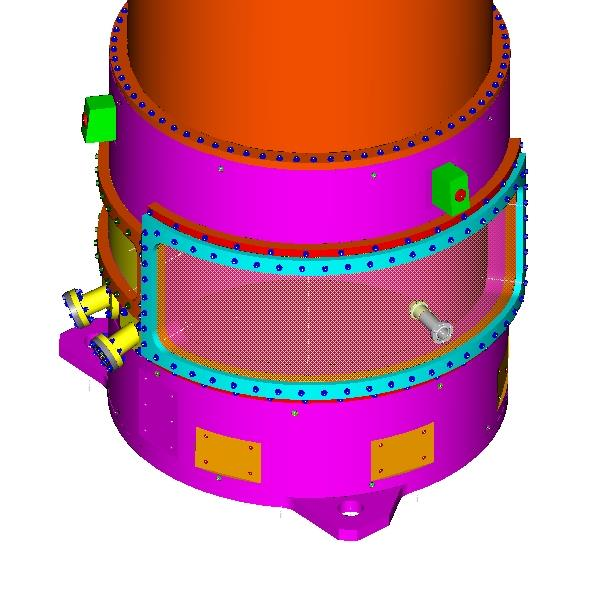
\includegraphics[width=\textwidth]{chap3/target_chamber.jpg}
        % \caption{X plane}
        \label{fig:target_chamber1}
    \end{subfigure}
    % \hfill
    \begin{subfigure}[b]{0.4\textwidth}
        \centering
        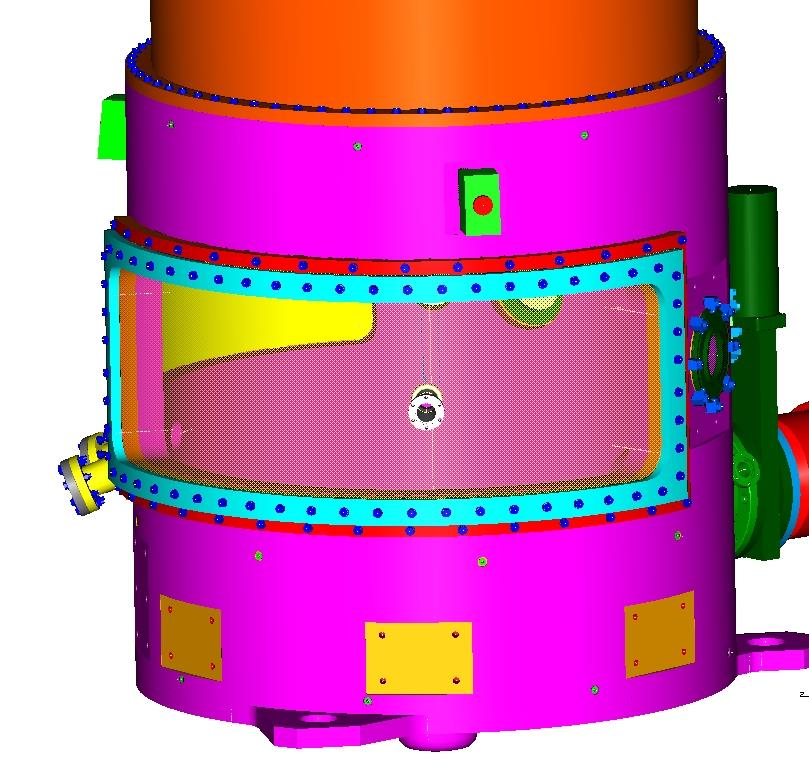
\includegraphics[width=\textwidth]{chap3/target_chamber2.jpg}
        % \caption{U plane}
        \label{fig:target_chamber2}
    \end{subfigure}
    \caption{The Hall  C target chamber.
             }
    \label{fig:target_chamber}
\end{figure}

\begin{figure}[h]
    \centering
    \begin{subfigure}[t]{0.3\textwidth}
        \centering
        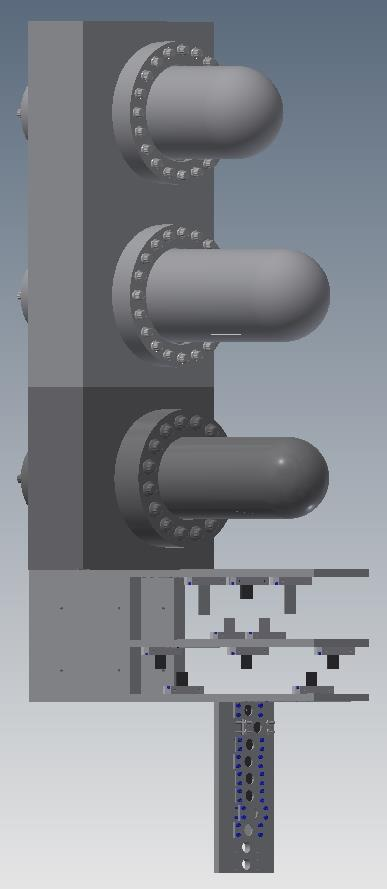
\includegraphics[height=3.5in]{chap3/target1.jpg}
        % \caption{}
        \label{fig:target_ladder1}
    \end{subfigure}
    \hfill
    \begin{subfigure}[t]{0.3\textwidth}
        \centering
        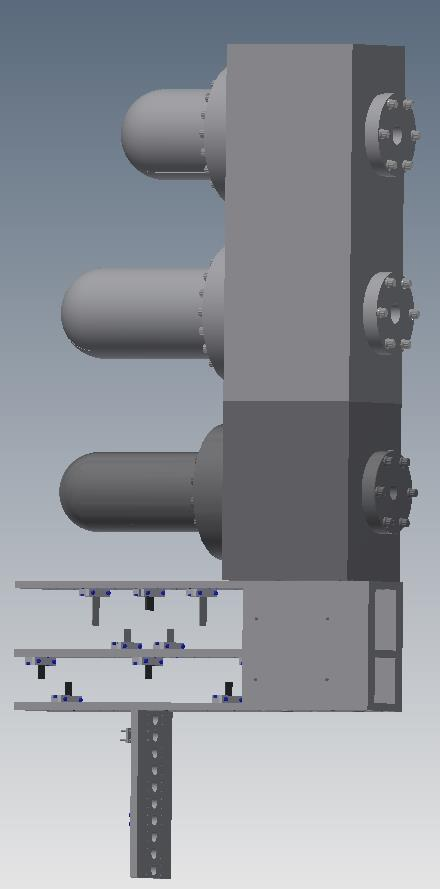
\includegraphics[height=3.5in]{chap3/target2.jpg}
        % \caption{}
        \label{fig:target_ladder2}
    \end{subfigure}
    \hfill
    \begin{subfigure}[t]{0.3\textwidth}
        \centering
        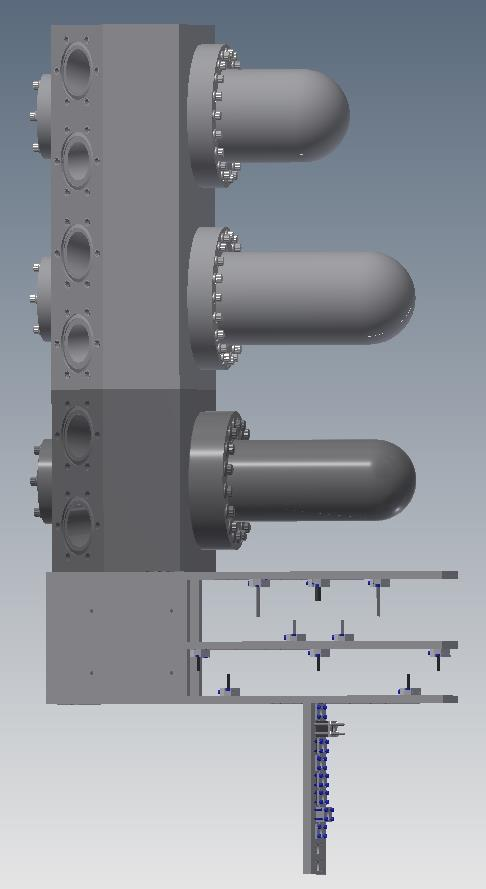
\includegraphics[height=3.5in]{chap3/target3.jpg}
        % \caption{}
        \label{fig:target_ladder3}
    \end{subfigure}
    \caption{The Hall C target ladder.
             }
    \label{fig:target_ladder}
\end{figure}

The target ladder contains three cryotarget loops, two ``dummy'' targets
consisting of two aluminum foils placed at z positions corresponding to the
entrance and exit windows of the cryotargets, two optics targets, and a number
of solid targets.
Table~\ref{tab:target_ladder_summary} summarizes the target ladder as
configured for the 2017 commissioning experiments, including our experiment,
E12-06-107.
During our experiment, cryotarget loop 1 was filled with \ch{LHe3}, loop 2
with \ch{LH2}, and loop 3 with \ch{LD2}.
The loops can be filled with other gases depending on experimental
requirements.

A detailed engineering drawing of the ladder is available online~\cite{target_drawing}.

\begin{table}[h]
    \centering
    \caption{Summary of the materials and thicknesses of the cryotarget loops and dummy targets.}
    \label{tab:target_ladder_summary}
    \begin{subtable}[h]{1.0\textwidth}
        \caption{Cryotarget loops and dummy targets}
        \resizebox{1.0\textwidth}{!}{
            \begin{tabular}[t]{lllll}
                \hline
                \hline
                Target          & Entrance Thickness [mm]  & Exit thickness [mm]     & Length [mm]     & Material  \\
                \hline
                Loop 1 (4 cm)   & $0.165 \pm 0.0019$       & $0.151 \pm 0.0053$ Tip  & $40  \pm 0.25$  & Aluminum 7075   \\ % tip
                                % &                          & $0.151 \pm 0.0097$ Wall &                 &           \\
                                                                                                                   % \\
                Loop 2 (10 cm)  & $0.104 \pm 0.0025$       & $0.133 \pm 0.0096$ Tip  & $10  \pm 0.26$  & Aluminum 7075   \\ % tip
                                % &                          & $0.162 \pm 0.014$ Wall  &                 &           \\
                                                                                                                   % \\
                Loop 3 (15 cm)  & $0.147 \pm 0.008$        & $0.177 \pm 0.013$ Tip   & $150 \pm 0.26$  & Aluminum 7075   \\ % tip
                                % &                          & $0.24  \pm 0.025$ Wall  &                 &           \\
                                                                                                                   % \\
                4 cm dummy      & $0.0789 \pm 0.000148$    & $0.0811 \pm 0.00014$    &                 & Aluminum 7075   \\
                                                                                                                   % \\
                10 cm dummy     & $0.1816 \pm 0.0003$      & $0.1815 \pm 0.0003$     &                 & Aluminum 7075   \\
                (with carbon foil at  & & & & \\
                z=0, described below) & & & & \\
                \hline
            \end{tabular}
            \label{table:target_ladder_cryo_summary1}
        } % resizebox
    \end{subtable}
    \vspace{1cm}
    \begin{subtable}[h]{1.0\textwidth}
        \caption{Optics and solid targets}
        \resizebox{1.0\textwidth}{!}{
            \begin{tabular}[t]{llcl}
                \hline
                \hline
                Target                 & Thickness [\si{\g\per\cm\squared}] & z position [cm] & Material  \\
                \hline
                Optics (three foils)   & $0.044  \pm 0.001$                  & -10, 0, +10     & Aluminum 7075/Carbon 99.95\%                         \\
                Optics (two foils)     & $0.044  \pm 0.001$                  & -5, +5          & Carbon 99.95\%                                       \\
                Carbon on 10 cm dummy  & $0.4426 \pm 0.0008$                 & 0               & Carbon 99.95\%                                       \\
                Carbon Hole            & $0.171  \pm 0.001$                  & 0               & Carbon 99.95\%                                       \\
                Carbon 6\%             & $2.068  \pm 0.004$                  & 0               & Carbon 99.95\%                                       \\
                Carbon 1.5\%           & $0.5244 \pm 0.001$                  & 0               & Carbon 99.95\%                                       \\
                Carbon 0.5\%           & $0.1749 \pm 0.00035$                & 0               & Carbon 99.95\%                                       \\
                \ch{^{10}B4C}          & $0.5722 \pm 0.001$                  & 0               & \ch{^{10}B4C} (99.9\% Chem/95\% enrichment)          \\
                \ch{^{11}B4C}          & $0.6348 \pm 0.001$                  & 0               & \ch{^{11}B4C} (99.9\% Chem/95\% enrichment)          \\
                \ch{BeO}               & $0.263  \pm 0.001$                  & 0               & \ch{BeO} 99.5\%                                      \\
                \hline
            \end{tabular}
            \label{table:target_ladder_cryo_summary2}
        } % resizebox
    \end{subtable}
\end{table}

Each cryotarget loop is maintained at \si{\sim3}{K} below the fluid's boiling
point by constantly recycling the fluid through a circuit containing the target
cell and a heat exchanger.

% TODO: Modify Greg's figure to reflect new cell geometry
\begin{figure}[!h]
    \centering
    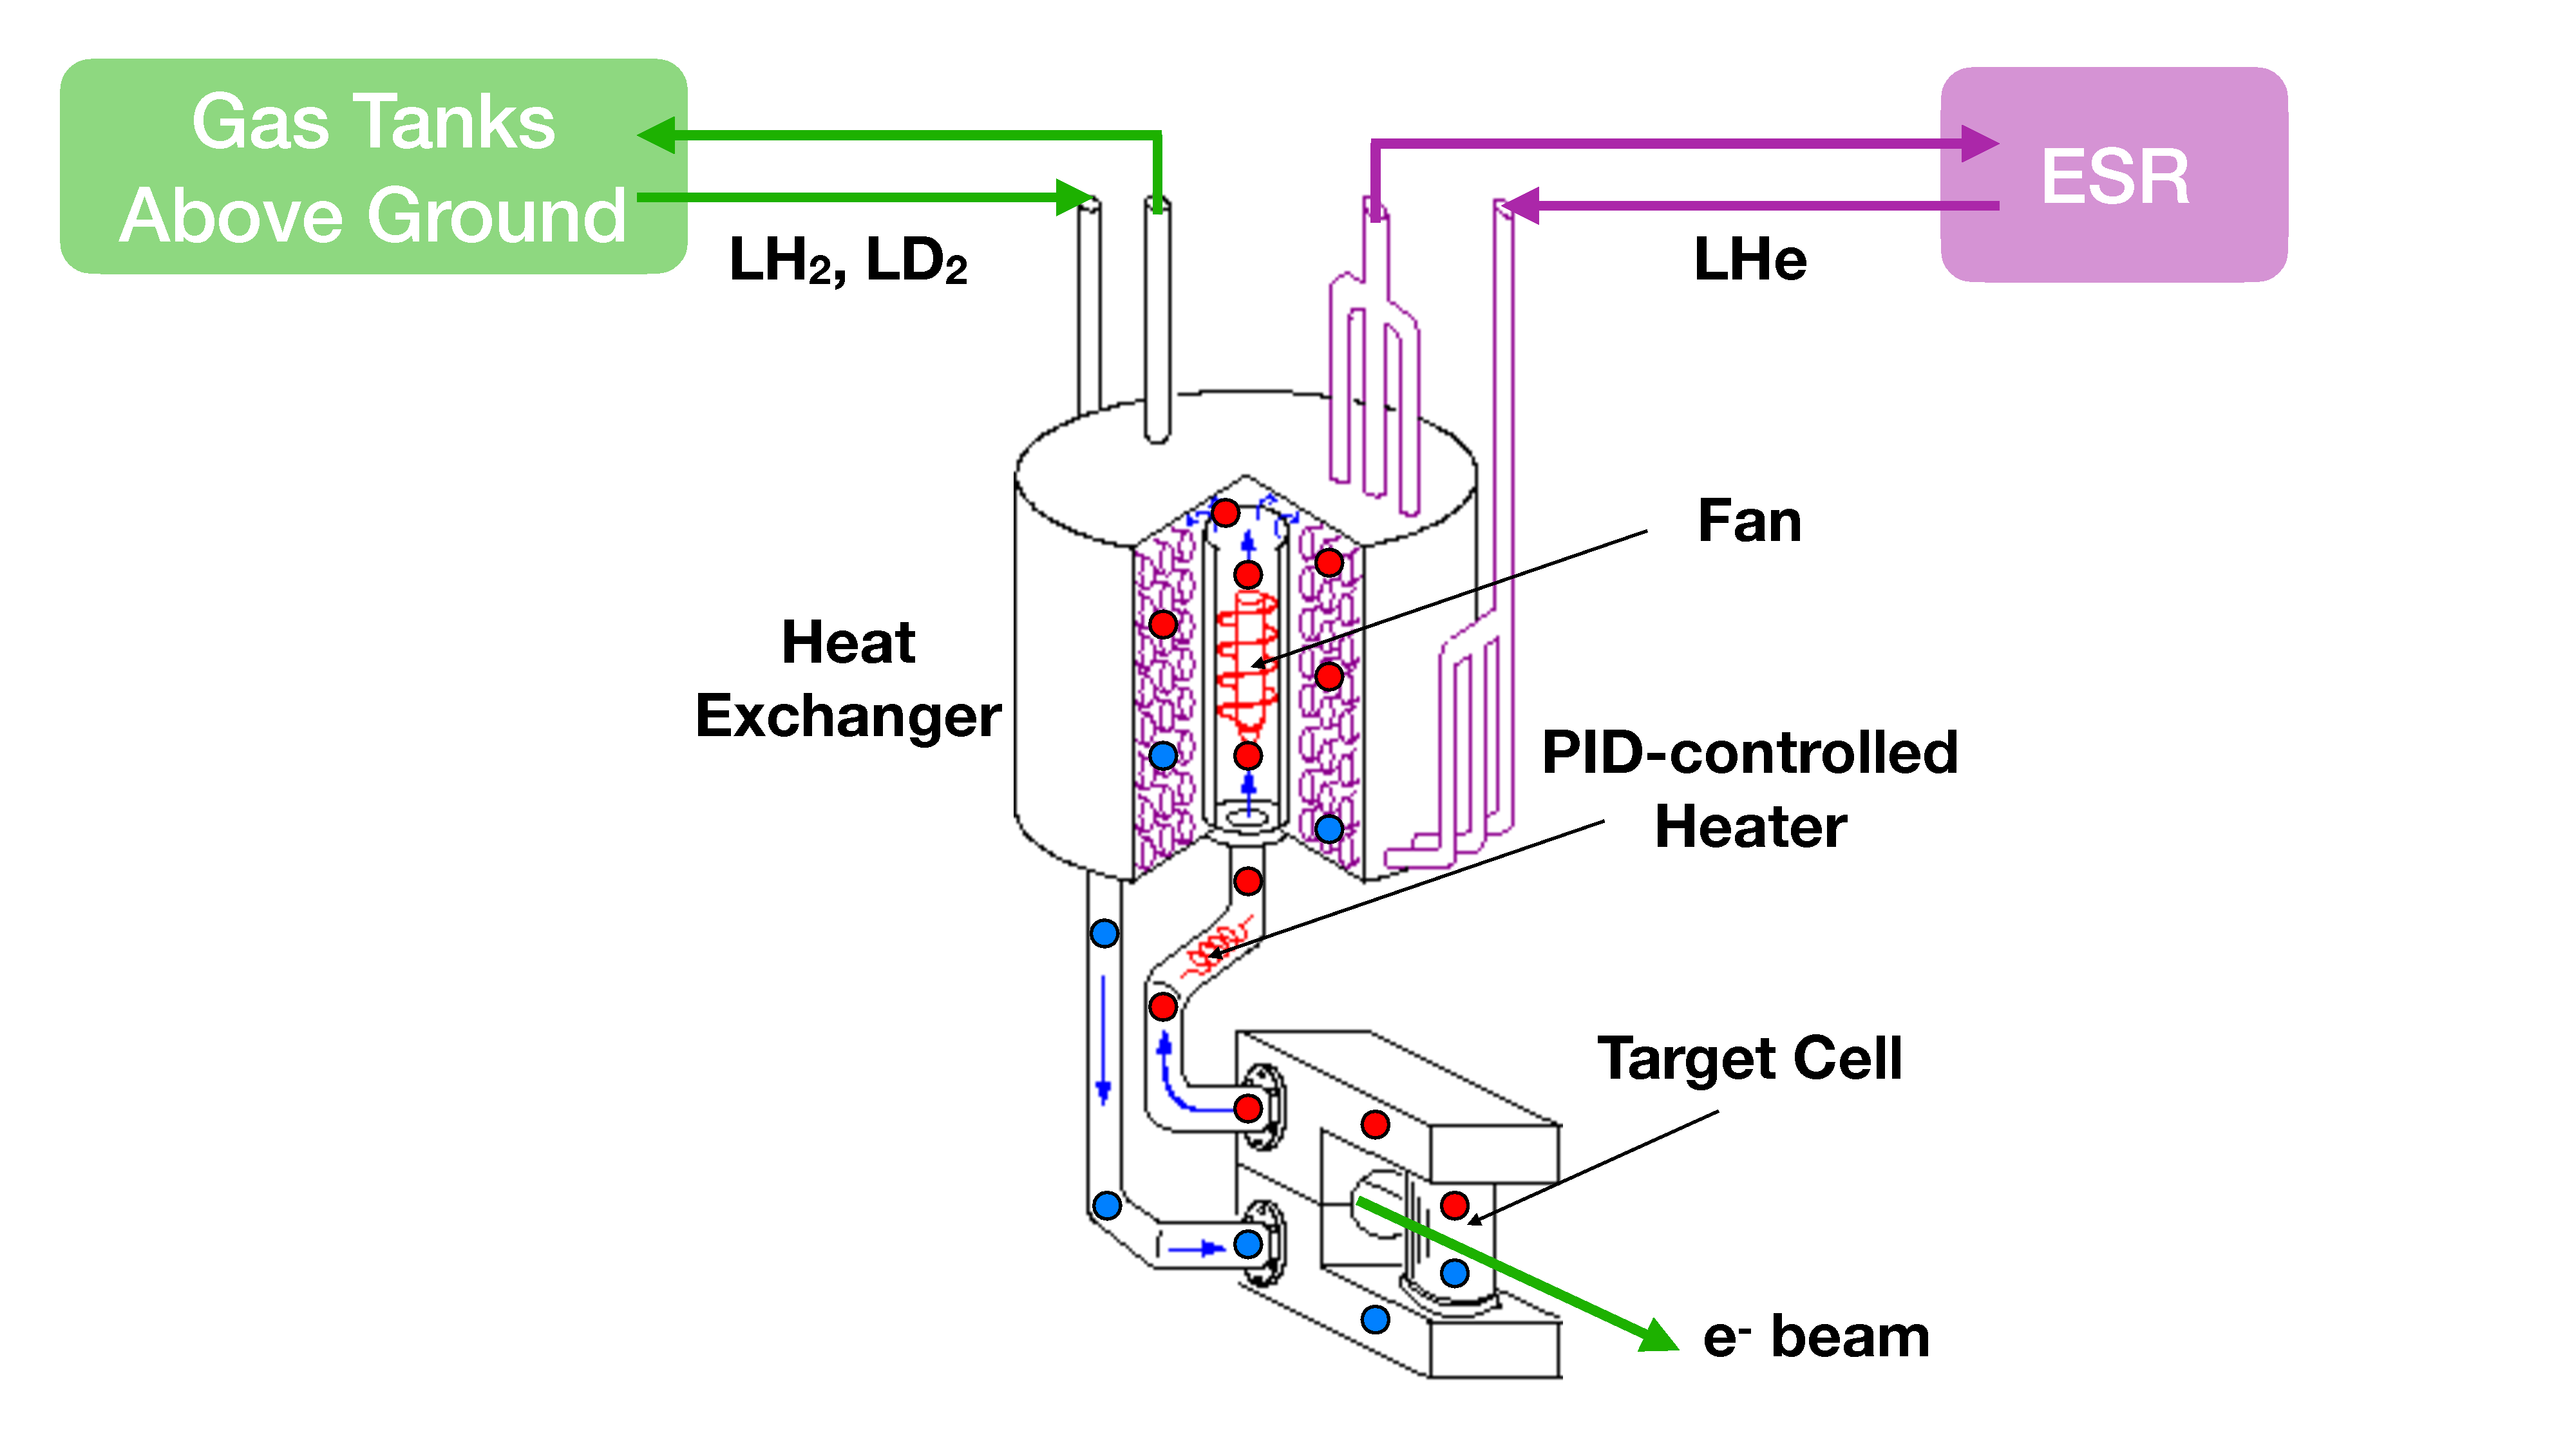
\includegraphics[width=1.0\textwidth]{chap3/target_cell_temperature_control.pdf}
    \caption{A cartoon of the system that maintains the cryotargets'
             temperatures.
            }
    \label{fig:cryotarget_temperature_regulation}
\end{figure}

A gas panel outside the counting house feeds a constant supply of target fluid
to the heat exchanger, where the \si{15}{K} liquid helium coolant from the End
Stage Refrigerator cools it to the target temperature of \si{\sim3}{K} below
boiling.
The fluid is then sent to the target cell which is  designed to maintain
uniform fluid velocity and density as the fluid makes its way from the cell's
inlet to its outlet.
As it leaves, the fluid will be at a higher temperature due to heat deposited
by the beam in operating conditions.
In the event that the beam is off, tripped, or otherwise interrupted, a high
power heater controlled by a software PID (Proportional-Integral-Derivative)
loop heats the exiting target fluid as if the beam were present.
The fluid then returns to the heat exchanger, completing the circuit.
